
\chapter{HARDroid: Reconocedor de Actividades Humanas}

\label{chap5:hardroid}

\section{Introducción}

\label{sec51:intro}En este capítulo introducimos un sistema que clasifica
la actividades humanas ambulatorias utilizando teléfonos móviles inteligentes
con la plataforma \emph{Android}\texttrademark: \emph{HARDroid}.
El sistema es una adaptación del diseño utilizado por sistemas existentes
como \emph{Google Play Services} \cite{Google2013l}, específicamente
la funcionalidad para reconocer actividades humanas utilizando los
conceptos y técnicas expuestos en capítulos precedentes. 

El sistema \emph{HARDroid} está implementado en base a dos componentes
principales: una interfaz de programación que expone las facilidades
y un servicio en ejecución que realiza las funciones principales del
sistema. La interfaz para programadores (\abbr{API}) proporciona
una firma de funciones bien definidas junto con la documentación adecuada
para que toda aplicación móvil de terceros utilice como un componente
externo la solución de un sistema \abbr{HAR}. El servicio de trasfondo
en la plataforma \emph{Android\texttrademark} es una aplicación para
teléfonos móvil independiente que implementa algoritmos de reconocimiento
de actividades humanas.

La propuesta de este trabajo se basa en un diseño desacoplado para
contar con una implementación genérica y extensible de un sistema
\abbr{HAR}. Como en todo sistema de \emph{software}, el diseño adecuado
posibilita la evolución y mantenimiento del mismo sin afectar el funcionamiento
de otras aplicaciones móviles clientes dependientes. 

Las siguientes secciones se organizan de la siguiente manera: primeramente
en la sección \ref{sec52:dise=0000F1o} damos una introducción de
las consideraciones de diseño y metodología utilizadas para la construcción
de los componentes de software. Se empieza con los conceptos generales
de Ingeniería de Software hasta concluir con los detalles técnicos
de la plataforma \emph{Android}. La siguiente sección \ref{sec53:arquitectura}
incluye una vista general del sistema explicando su arquitectura.
La sección \ref{sec54:hardroid} conforma el núcleo principal de este
proyecto donde una implementación \abbr{HAR} en forma de aplicación
móvil desacoplado es presentado. También, en la sección \ref{sec55:activity}
se explica el desenvolvimiento de una herramienta para realizar experimentos
y evaluar los resultados asociados a la solución. Por último, en la
sección \ref{sec56:conclusion} se discuten los resultados preliminar
obtenidos como motivo de los componentes de software construidos.

\section{Diseño General}

\label{sec52:dise=0000F1o}La construcción del sistema \emph{HARDroid
}está enmarcado dentro del ecosistema de aplicaciones móviles. Desde
el punto de vista conceptual del desarrollo de aplicaciones móviles
es necesario enfocarse en dos aspectos principales para el diseño:
el medio y el contexto.

Una aplicación móvil puede presentarse en diversos medios que corresponden
con el enfoque técnico \cite{Fling2009}, es decir: un sitio Web Móvil,
una aplicación Web Móvil, SMS, Juegos, herramientas\emph{ Widgets}
y aplicaciones nativas. Las aplicaciones nativas son uno de los medios
más utilizados debido a la rica experiencia de usuario y capacidades
que pueden ser explotadas en los dispositivos, ya que disponen de
gran soporte en la plataforma subyacente. Por ejemplo, en la plataforma
para teléfonos móviles \emph{Android }se dispone de las capacidades
disponibles del dispositivo como almacenamiento, ubicación, sensores
y además un medio de distribución certificado como ser el \emph{Google
Play Store} \cite{Google2016p}. 

Por otro lado, está el contexto de la aplicación que se refiere a
la experiencia que el usuario final obtiene al utilizar el sistema
móvil. Para esto el sistema móvil procesa la información de contexto
que rodea al usuario dando una interacción distinta a los sistemas
convencionales. A continuación se listan los tipos de contexto comunes
utilizados en las aplicaciones móviles y un breve ejemplo de su funcionalidad
\cite{Fling2009}:
\begin{itemize}
\item \emph{Utilidad}: Calculadora, Conversión de monedas.
\item \emph{Localización}: Mapas, Registro de actividades físicas.
\item \emph{Informativo}: Buscar información relevante.
\item \emph{Productividad}: Comprar productos y pagar servicios
\item \emph{Inmersión}: Juegos 
\end{itemize}
Estos tipos de contexto se pueden combinar para crear mejores experiencias
de uso de la aplicación móvil. El trabajo desarrollado en esta tesis
se adecua al modelo de aplicaciones móviles de contexto. Se busca
proveer un componente de \emph{Utilidad} que puede ser combinado con
diferentes aplicaciones móviles desarrollados por terceros y pueda
ser mantenido de forma colaborativa. 

\subsection{Criterios de diseño}

La implementación de este trabajo, así como la mayoría de los sistemas
de información, se rige bajo el principio de diseño \emph{basado en
componentes} donde se busca separar la complejidad de un sistema en
módulos y que estos interactúen entre sí. Los módulos en el diseño
de sistemas mejoran la flexibilidad y comprensión mientras se reduce
el tiempo de desarrollo de los mismos \cite{Parnas1972}.

Una de las técnicas más comunes de diseño de sistemas\emph{ }es la
separación por capas (\emph{Layering}) para dividir un sistema complejo
\cite{Fowler2002} en diferentes niveles. 

\subsubsection{Arquitecturas en capas}

Cuando un sistema se construye en términos de capas, los módulos se
organizan en niveles apilados como en un pastel, donde cada capa se
soporta sobre la capa baja subyacente. En este sentido, la capa superior
utiliza varios servicios definidos en capas inferiores, pero la capa
inferior desconoce y no depende de las capas en niveles superiores.
Las capas definen concretamente las responsabilidades y encapsulan
las funcionalidades soportadas en cada nivel.

La popularidad de la división de sistemas en módulos por capas se
volvió más relevante con el auge de los sistemas tipo \emph{Cliente-Servidor}.
Estos sistemas fueron inicialmente concebidos como de dos (2) capas:
el cliente se encarga de la interfaz de usuario y la lógica de la
aplicación, y el servidor usualmente es una bases de datos relacional.
En la \figref{fig5:cliente_servidor} se muestra una representación
de la arquitectura en dos capas. Para sistemas sencillos que desplieguen
información y actualicen datos, este modelo es el más adecuado. Sin
embargo, a medida que se construyen sistemas más complejos, el problema
radica mantener la lógica central del sistema: las reglas de negocio,
validaciones, cálculos, etc. El modelo de dos capas propone ubicar
la lógica central embebida en la interacciones de la Interfaz de Usuario
(capa cliente) o almacenar los mismos en procedimientos almacenados
en la basa de datos (capa servidor).

\begin{figure}[h]
\begin{centering}
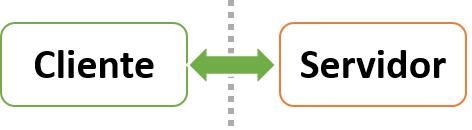
\includegraphics[width=0.5\columnwidth]{capitulo-5/graphics/cliente_servidor}
\par\end{centering}
\caption[Modelo de dos capas]{\label{fig5:cliente_servidor}Modelo de dos capas}
\end{figure}

Debido a las limitaciones del enfoque Cliente-Servidor, se puede extender
el mismo con la ayuda del paradigma de Orientación a Objetos para
construir sistemas con arquitecturas de tres (3) capas. Estas capas
son comúnmente conocidas como \cite{Fowler2002}: Presentación, Dominio
y Recursos. En la \tabref{tab5:tres_capas} se definen las responsabilidades
correspondientes a cada capa. 

\begin{table}
\begin{centering}
\begin{tabular}[t]{|l|>{\raggedright}p{0.5\columnwidth}|}
\hline 
Capa & Responsabilidades\tabularnewline
\hline 
\hline 
Presentación & Provisión de servicios a sistemas externos, despliegue de información
e interacción con el usuario.\tabularnewline
\hline 
Dominio & \multirow{1}{0.5\columnwidth}{Lógica y procesamiento del sistema.}\tabularnewline
\hline 
Recursos & Comunicación con bases de datos, sistemas externos, integración, transacciones
y otros componentes.\tabularnewline
\hline 
\end{tabular}
\par\end{centering}
\caption[Modelo de tres capas]{\label{tab5:tres_capas}Modelo de tres capas}
\end{table}

Independientemente del tipo de sistema de información a ser construido
dividir el mismo en capas lógicas, dividir el sistema en partes separadas,
permite reducir el acoplamiento entre diferentes módulos, inclusive
si todos los módulos se ejecutan en la misma máquina física. En la
\figref{fig5:tres_capas} se muestra la arquitectura de tres capas
discutida anteriormente.

\begin{figure}[h]
\begin{centering}
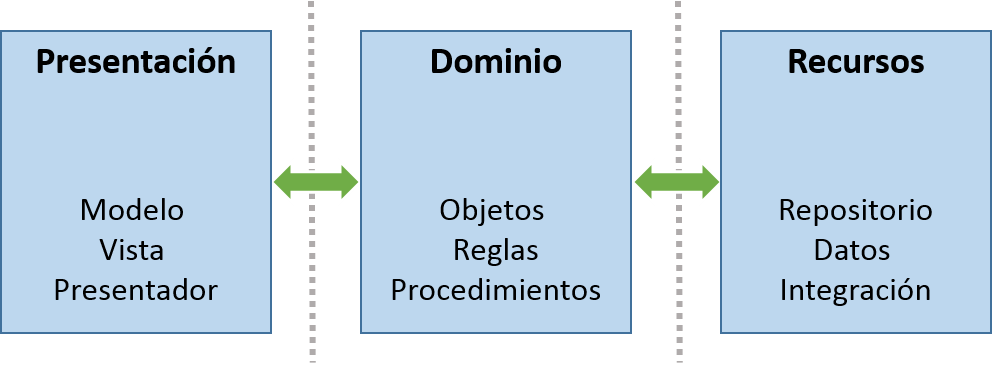
\includegraphics[width=0.8\textwidth]{capitulo-5/graphics/arqui_tres_capas}
\par\end{centering}
\caption[Modelo de tres capas]{\label{fig5:tres_capas}Modelo de tres capas}

\end{figure}


\subsubsection{Patrones de diseño}

Los patrones de diseño son parte del paradigma de orientación a objetos
ideados para solucionar problemas comunes determinados en un contexto
particular \cite{Shalloway2004}. Una definición acertada se cita
a continuación.
\begin{quotation}
<<\emph{Cada patrón describe un problema que ocurre una y otra vez
en nuestro entorno, y también describe la solución principal al problema,
de tal manera que la solución pueda ser utilizada millares de veces,
sin tener que duplicar el trabajo de pensar cómo resolver el problema.>>}
\cite{Alexander1977}
\end{quotation}
Para nuestro objetivo de implementación, se utilizan los patrones
de diseño para organizar el \emph{Dominio}, la lógica principal del
sistema. La metodología de dividir el\emph{ Dominio} por medio de
los patrones \cite{Fowler2002}:
\begin{enumerate}
\item \emph{Service Layer}: capa de servicios
\item \emph{Domain Model}: modelo del dominio
\end{enumerate}
La capa de servicios es el punto de interacción entre la \emph{Presentación}
y el\emph{ Dominio}, por lo que actúa como proveedor de una interfaz
clara (comúnmente una \abbr{API}). Este patrón define los límites
del sistema con una capa de servicios que establece el conjunto de
operaciones disponibles y coordina el proceso de cada operación. La
capa de servicios puede ser tan gruesa como tan fina como se requiera,
esta puede contener objetos de servicio con reglas de negocio, manejo
de transacciones y seguridad.

Por otro lado, el modelo del dominio da soporte a la capa de servicios.
Este patrón define objetos de dominio que tienen incorporados datos
y comportamiento, estos representan de manera significativa el dominio
del problema a resolver. Debido a que la lógica de negocio de un sistema
puede ser bastante compleja. Estos objetos están diseñados para manejar
las diversas combinaciones de reglas y lógica del sistema.

\subsubsection{Guías Generales}

En general las guías generales para construcción de sistemas orientados
a objetos fueron utilizados en este trabajo. Algunos de los principios
más relevantes que han sido considerados son \cite{Albin2003}:
\begin{itemize}
\item Modularidad
\item Orientación a Objetos
\item Reusabilidad
\item Ocultamiento de Información
\item Abstracción
\end{itemize}
Siguiendo estos principios se ha logrado un desarrollo exitoso en
la implementación de los componentes y aplicaciones móviles. Además,
se ha enfocado el desarrollo con miras a la colaboración basada en
la comunidad de código abierto Licencia Pública Apache, Versión 2.0
(\emph{Apache License, Version 2.0}) \cite{GimenezYegros2016c}.

\subsection{Metodología de desarrollo}

\subsection{Tecnología }

\subsubsection{Android\texttrademark}

\paragraph{Arquitectura}

\paragraph{Componentes}

\subsection{Binder IPC}

\section{Arquitectura del proyecto}

\label{sec53:arquitectura}

\section{HARDroid: Servicio de Reconocimiento de Actividades}

\label{sec54:hardroid}

\subsection{Librería API}

\subsection{Servicio BINDER}

\subsection{Clasificador DEX}

\section{ActivitySurvey: Aplicación de Encuesta}

\label{sec55:activity}

\section{Conclusión}

\label{sec56:conclusion}
